\documentclass[english,man]{apa6}

\usepackage{amssymb,amsmath}
\usepackage{ifxetex,ifluatex}
\usepackage{fixltx2e} % provides \textsubscript
\ifnum 0\ifxetex 1\fi\ifluatex 1\fi=0 % if pdftex
  \usepackage[T1]{fontenc}
  \usepackage[utf8]{inputenc}
\else % if luatex or xelatex
  \ifxetex
    \usepackage{mathspec}
    \usepackage{xltxtra,xunicode}
  \else
    \usepackage{fontspec}
  \fi
  \defaultfontfeatures{Mapping=tex-text,Scale=MatchLowercase}
  \newcommand{\euro}{€}
\fi
% use upquote if available, for straight quotes in verbatim environments
\IfFileExists{upquote.sty}{\usepackage{upquote}}{}
% use microtype if available
\IfFileExists{microtype.sty}{\usepackage{microtype}}{}
\usepackage{color}
\usepackage{fancyvrb}
\newcommand{\VerbBar}{|}
\newcommand{\VERB}{\Verb[commandchars=\\\{\}]}
\DefineVerbatimEnvironment{Highlighting}{Verbatim}{commandchars=\\\{\}}
% Add ',fontsize=\small' for more characters per line
\usepackage{framed}
\definecolor{shadecolor}{RGB}{248,248,248}
\newenvironment{Shaded}{\begin{snugshade}}{\end{snugshade}}
\newcommand{\KeywordTok}[1]{\textcolor[rgb]{0.13,0.29,0.53}{\textbf{#1}}}
\newcommand{\DataTypeTok}[1]{\textcolor[rgb]{0.13,0.29,0.53}{#1}}
\newcommand{\DecValTok}[1]{\textcolor[rgb]{0.00,0.00,0.81}{#1}}
\newcommand{\BaseNTok}[1]{\textcolor[rgb]{0.00,0.00,0.81}{#1}}
\newcommand{\FloatTok}[1]{\textcolor[rgb]{0.00,0.00,0.81}{#1}}
\newcommand{\ConstantTok}[1]{\textcolor[rgb]{0.00,0.00,0.00}{#1}}
\newcommand{\CharTok}[1]{\textcolor[rgb]{0.31,0.60,0.02}{#1}}
\newcommand{\SpecialCharTok}[1]{\textcolor[rgb]{0.00,0.00,0.00}{#1}}
\newcommand{\StringTok}[1]{\textcolor[rgb]{0.31,0.60,0.02}{#1}}
\newcommand{\VerbatimStringTok}[1]{\textcolor[rgb]{0.31,0.60,0.02}{#1}}
\newcommand{\SpecialStringTok}[1]{\textcolor[rgb]{0.31,0.60,0.02}{#1}}
\newcommand{\ImportTok}[1]{#1}
\newcommand{\CommentTok}[1]{\textcolor[rgb]{0.56,0.35,0.01}{\textit{#1}}}
\newcommand{\DocumentationTok}[1]{\textcolor[rgb]{0.56,0.35,0.01}{\textbf{\textit{#1}}}}
\newcommand{\AnnotationTok}[1]{\textcolor[rgb]{0.56,0.35,0.01}{\textbf{\textit{#1}}}}
\newcommand{\CommentVarTok}[1]{\textcolor[rgb]{0.56,0.35,0.01}{\textbf{\textit{#1}}}}
\newcommand{\OtherTok}[1]{\textcolor[rgb]{0.56,0.35,0.01}{#1}}
\newcommand{\FunctionTok}[1]{\textcolor[rgb]{0.00,0.00,0.00}{#1}}
\newcommand{\VariableTok}[1]{\textcolor[rgb]{0.00,0.00,0.00}{#1}}
\newcommand{\ControlFlowTok}[1]{\textcolor[rgb]{0.13,0.29,0.53}{\textbf{#1}}}
\newcommand{\OperatorTok}[1]{\textcolor[rgb]{0.81,0.36,0.00}{\textbf{#1}}}
\newcommand{\BuiltInTok}[1]{#1}
\newcommand{\ExtensionTok}[1]{#1}
\newcommand{\PreprocessorTok}[1]{\textcolor[rgb]{0.56,0.35,0.01}{\textit{#1}}}
\newcommand{\AttributeTok}[1]{\textcolor[rgb]{0.77,0.63,0.00}{#1}}
\newcommand{\RegionMarkerTok}[1]{#1}
\newcommand{\InformationTok}[1]{\textcolor[rgb]{0.56,0.35,0.01}{\textbf{\textit{#1}}}}
\newcommand{\WarningTok}[1]{\textcolor[rgb]{0.56,0.35,0.01}{\textbf{\textit{#1}}}}
\newcommand{\AlertTok}[1]{\textcolor[rgb]{0.94,0.16,0.16}{#1}}
\newcommand{\ErrorTok}[1]{\textcolor[rgb]{0.64,0.00,0.00}{\textbf{#1}}}
\newcommand{\NormalTok}[1]{#1}

% Table formatting
\usepackage{longtable, booktabs}
\usepackage{lscape}
% \usepackage[counterclockwise]{rotating}   % Landscape page setup for large tables
\usepackage{multirow}		% Table styling
\usepackage{tabularx}		% Control Column width
\usepackage[flushleft]{threeparttable}	% Allows for three part tables with a specified notes section
\usepackage{threeparttablex}            % Lets threeparttable work with longtable

% Create new environments so endfloat can handle them
% \newenvironment{ltable}
%   {\begin{landscape}\begin{center}\begin{threeparttable}}
%   {\end{threeparttable}\end{center}\end{landscape}}

\newenvironment{lltable}
  {\begin{landscape}\begin{center}\begin{ThreePartTable}}
  {\end{ThreePartTable}\end{center}\end{landscape}}

  \usepackage{ifthen} % Only add declarations when endfloat package is loaded
  \ifthenelse{\equal{\string man}{\string man}}{%
   \DeclareDelayedFloatFlavor{ThreePartTable}{table} % Make endfloat play with longtable
   % \DeclareDelayedFloatFlavor{ltable}{table} % Make endfloat play with lscape
   \DeclareDelayedFloatFlavor{lltable}{table} % Make endfloat play with lscape & longtable
  }{}%



% The following enables adjusting longtable caption width to table width
% Solution found at http://golatex.de/longtable-mit-caption-so-breit-wie-die-tabelle-t15767.html
\makeatletter
\newcommand\LastLTentrywidth{1em}
\newlength\longtablewidth
\setlength{\longtablewidth}{1in}
\newcommand\getlongtablewidth{%
 \begingroup
  \ifcsname LT@\roman{LT@tables}\endcsname
  \global\longtablewidth=0pt
  \renewcommand\LT@entry[2]{\global\advance\longtablewidth by ##2\relax\gdef\LastLTentrywidth{##2}}%
  \@nameuse{LT@\roman{LT@tables}}%
  \fi
\endgroup}


  \usepackage{graphicx}
  \makeatletter
  \def\maxwidth{\ifdim\Gin@nat@width>\linewidth\linewidth\else\Gin@nat@width\fi}
  \def\maxheight{\ifdim\Gin@nat@height>\textheight\textheight\else\Gin@nat@height\fi}
  \makeatother
  % Scale images if necessary, so that they will not overflow the page
  % margins by default, and it is still possible to overwrite the defaults
  % using explicit options in \includegraphics[width, height, ...]{}
  \setkeys{Gin}{width=\maxwidth,height=\maxheight,keepaspectratio}
\ifxetex
  \usepackage[setpagesize=false, % page size defined by xetex
              unicode=false, % unicode breaks when used with xetex
              xetex]{hyperref}
\else
  \usepackage[unicode=true]{hyperref}
\fi
\hypersetup{breaklinks=true,
            pdfauthor={},
            pdftitle={Using Beta Regression to Model Normative Aspects of Prejudice and Political Attitudes},
            colorlinks=true,
            citecolor=blue,
            urlcolor=blue,
            linkcolor=black,
            pdfborder={0 0 0}}
\urlstyle{same}  % don't use monospace font for urls

\setlength{\parindent}{0pt}
%\setlength{\parskip}{0pt plus 0pt minus 0pt}

\setlength{\emergencystretch}{3em}  % prevent overfull lines

\ifxetex
  \usepackage{polyglossia}
  \setmainlanguage{}
\else
  \usepackage[english]{babel}
\fi

% Manuscript styling
\captionsetup{font=singlespacing,justification=justified}
\usepackage{csquotes}
\usepackage{upgreek}



\usepackage{tikz} % Variable definition to generate author note

% fix for \tightlist problem in pandoc 1.14
\providecommand{\tightlist}{%
  \setlength{\itemsep}{0pt}\setlength{\parskip}{0pt}}

% Essential manuscript parts
  \title{Using Beta Regression to Model Normative Aspects of Prejudice and
Political Attitudes}

  \shorttitle{Beta Regression}


  \author{Mark H. White II\textsuperscript{1}}

  \def\affdep{{""}}%
  \def\affcity{{""}}%

  \affiliation{
    \vspace{0.5cm}
          \textsuperscript{1} University of Kansas  }

  \authornote{
    \newcounter{author}
    I would like to thank Dr.~Achim Zeileis and Dr.~Jonathan Templin for
    comments on an earlier version of this manuscript. All code and data
    necessary to reproduce this manuscript can be accessed at
    \url{https://github.com/markhwhiteii/beta_hurdle}.

                      Correspondence concerning this article should be addressed to Mark H. White II. E-mail: \href{mailto:markhwhiteii@gmail.com}{\nolinkurl{markhwhiteii@gmail.com}}
                }


  \abstract{Many important phenomena in the psychological study of prejudice and
political attitudes involve measuring dependent variables that are
strongly influenced by normative pressures. Norms produce invariance,
which can create outcome variables with ceiling effects, floor effects,
and heteroskedasticity. These characteristics cause problems for
ordinary least squares (OLS) regression and analysis of variance
(ANOVA), which assume conditional normality and constant variance. I
describe the beta distribution and propose beta regression as a way to
model doubly-bounded continuous variables (e.g., Likert scales, feeling
thermometers). I also demonstrate how beta regression can model
conditional variance, ceiling effects, and floor effects as a proxy for
norms. Lastly, I provide a brief tutorial on how to implement various
beta regression models using R.}
  \keywords{beta regression, hurdle models, gamlss, norms, social attitudes \\

    
  }





\usepackage{amsthm}
\newtheorem{theorem}{Theorem}
\newtheorem{lemma}{Lemma}
\theoremstyle{definition}
\newtheorem{definition}{Definition}
\newtheorem{corollary}{Corollary}
\newtheorem{proposition}{Proposition}
\theoremstyle{definition}
\newtheorem{example}{Example}
\theoremstyle{remark}
\newtheorem*{remark}{Remark}
\begin{document}

\maketitle

\setcounter{secnumdepth}{0}



Behavior is a function of the person and the environment (Lewin, 1951).
It is important that researchers study the effects of personality
\emph{and} situational variables, as well as how they interact. However,
Louis, Mavor, and Terry (2003) argue that \enquote{normative influence
in social attitudes and behavior is systematically underestimated}
(p.~190). The logic behind this argument is that researchers use
statistical procedures that analyze \emph{variance} and assume
normality. But norms produce \emph{invariance}---they lead people to
engage in the same behaviors or respond to survey items in the same way.
Norms can produce skewed distributions, as well: floor effects (strong
norm in disagreement with a survey item), ceiling effects (strong norm
for agreement), or strongly leptokurtic distributions (strong norm for
answering the midpoint).

Louis and colleagues note that using only the limited number of common
statistical procedures (e.g., ordinary least squares, OLS, regression)
influences theoretical and methodological choices: Researchers look for
measures that are normally distributed, which they argue favors
personality explanations and \enquote{privileges measures that tap
unclear or weak norms} (p.~190). This systematically ignores phenomena
that are subject to strong normative influences, which overestimates the
influence of personality on attitudes and behavior.

When personality researchers \emph{do} model these types of variables
using OLS regression, it is the deviant cases that drive the linear
relationships. For example, Louis et al. (2003) examine the bivariate
relationship between right-wing authoritarianism (RWA) and how much
people agree with the item, \enquote{The White race is the best race.}
72\% of the sample selected \enquote{1, \emph{Strongly Disagree}} to the
White race item. However, what often gets reported in articles is just
the correlation: \(r = .34\), \(p < .001\). We learn that RWA positively
predicts White supremacist attitudes. But what are we missing when only
this is reported?

Louis et al. note that, for 72\% of the sample, a correlation can not
even be calculated---there was no variance in the scores. Everyone in
this 72\% adhered to the egalitarian norm that it is not OK to openly
say the White race is the best race. For the rest of the sample, the
correlation was \(.19\). The authors raise two concerns: first, that
researchers could decide to exclude items like this because they aren't
normally distributed, which prevents one from studying an important
construct (White supremacy); second, readers interpret correlations
symmetrically. A \enquote{symmetric} interpretation is that people at
\emph{both} the high and low ends of the authoritarianism spectrum are
driving the relationship, when we know that is only the top 28\% of the
sample.

\subsection{Aims of the Present Paper}\label{aims-of-the-present-paper}

I second the concerns raised by Louis et al. (2003). The purpose of this
paper is to propose a concrete solution to the issues raised. They
lamented that there is \enquote{no conventional analysis of invariance}
(p.~192), and they gave no suggestions for how else to analyze data to
mitigate these issues. I propose beta regression (presented a year after
Louis and colleages' paper) as one solution. Smithson and Verkuilen
(2006) touch on this briefly, but I fully extend the argument here.

I have three goals in the present paper: first, to familiarize
researchers with the beta distribution and beta regression, which can
handle non-normal data and model conditional variance; second, to
empirically demonstrate Louis et al.'s contention that norms produce
invariance; third, to give a brief tutorial on how researchers can use
beta regression to address the crucial issues raised by Louis et al.
(2003), such as modeling normative aspects in survey responses.

\section{Statistical Background}\label{statistical-background}

\subsection{The Beta Distribution}\label{the-beta-distribution}

The beta distribution can be used in a generalized linear model when the
values of the dependent variable are bounded \(0 < y < 1\) (Coxe, West,
\& Aiken, 2013). The probability density function (pdf) of the beta
distribution is determined by two parameters, \(\alpha\) and \(\beta\),
that are called \enquote{shape} parameters:

\begin{center}
$f(y;\alpha,\beta)={\Gamma(\alpha+\beta)\over\Gamma(\alpha)\Gamma(\beta)}y^{\alpha-1}(1-y)^{\beta-1}$
\end{center}

where \(\Gamma(.)\) is the gamma function. One of the benefits of the
beta distribution is that it is flexible and can take a number of
distributional shapes (Figure 1).

\begin{figure}
\centering
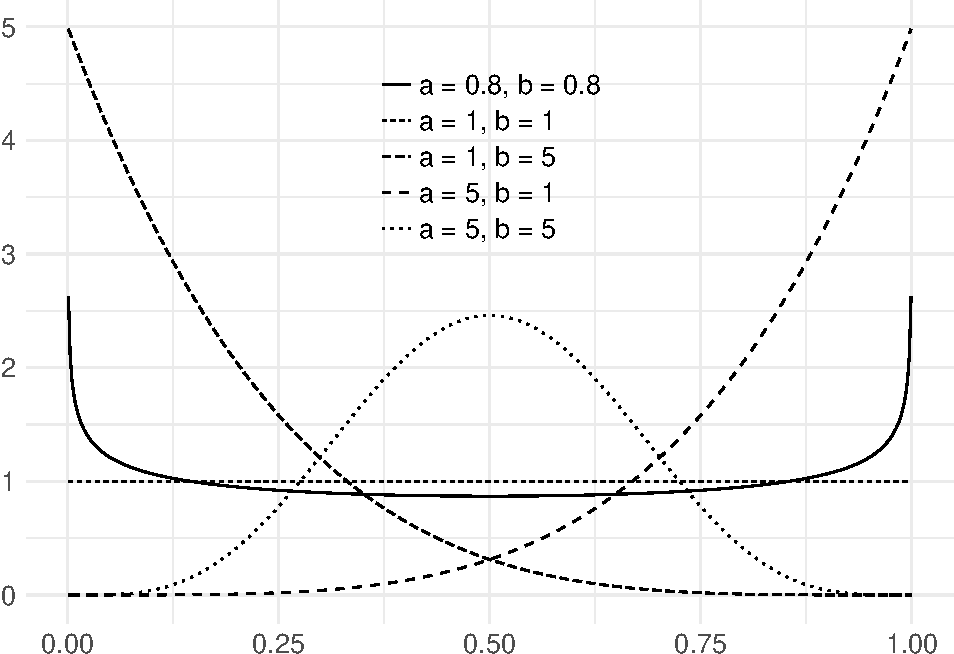
\includegraphics{beta_hurdle_files/figure-latex/unnamed-chunk-2-1.pdf}
\caption{\label{fig:unnamed-chunk-2}Beta probability density functions with
various combinations of shape parameters.}
\end{figure}

These parameters are not inherently meaningful to researchers. Rigby,
Stasinopoulos, Heller, and De Bastiani (2017) \enquote{reparameterized}
the beta distribution so that the two parameters determining the shape
of the distribution would be more useful in a regression framework (see
Ferrari \& Cribari-Neto, 2004 for a different parameterization). Instead
of predicting \(\alpha\) and \(\beta\), they parameterize (i.e.,
algebraically rearrange parameters) the distribution so that beta
regression predicts two different parameters: \(\mu\) (called the
\enquote{location} parameter) and \(\sigma\) (called the \enquote{scale}
parameter), where \(\mu={\alpha\over(\alpha+\beta)}\) and
\(\sigma=\sqrt{1\over(\alpha+\beta+1)}\). \(\mu\) is equivalent to the
mean, and \(\sigma\) is related positively to the variance (note that
\(\sigma\) is \emph{not} the standard deviation, even though \(\sigma\)
commonly refers to the standard deviation). The variance is equivalent
to \(\sigma^2\mu(1-\mu)\). There are two things to note from this
equation: first, the greater the \(\sigma\), the greater the variance;
second, the variance depends on the mean, which means that beta
regression will be naturally heteroskedastic (covered shortly). Using
this distribution in a regression framework cannot handle the dependent
variable taking on values 0 and 1, however. How can we model dependent
variables in the range \(0 \leq y \leq 1\)?

\subsection{Zero-One Inflated Beta
Distribution}\label{zero-one-inflated-beta-distribution}

Rigby et al. (2017) show that the beta distribution can be
\enquote{inflated} at 0 and 1, meaning the dependent variable contains
0s and 1s (i.e., \(0 \leq y \leq 1\)), the pdf for this beta inflated
distribution, \(\text{beinf}\), is:

\begin{center}
\[
\text{beinf}(y;\mu,\sigma,\nu,\tau) =
\begin{cases}
  p_0                             & \text{if } y = 0\\
  (1 - p_0 - p_1)f(y;\mu,\sigma)  & \text{if } 0 < y < 1\\
  p_1                             & \text{if } y = 1
\end{cases}
\]
\end{center}

for \(0 \leq y \leq 1\), where \(f(y;\mu,\sigma)\) is the beta pdf with
\(\mu\) and \(\sigma\) bounded \emph{between} 0 and 1 The two additional
parameters, \(\nu\) and \(\tau\), are related to \(p_0\) and \(p_1\),
respectively. \(p_0\) is the probability that a case equals 0, \(p_1\)
is the probability that a case equals 1, and \(p_2\) (i.e.,
\(1 - p_0 - p_1\)) is the probability that the case comes from the beta
distribution. In terms of these two additional parameters,
\(p_0 = {\nu \over (1 + \nu + \tau)}\) and
\(p_1 = {\tau \over (1 + \nu + \tau)}\). Rearranging these
algebraically, \(\nu\) is the odds that a case is 0 to being
\(0 < y < 1\), \(\nu = p_0 / p_2\), and \(\tau\) is the odds that a case
is a 1 to being \(0 < y < 1\), \(\tau = p_1 / p_2\). It should be noted,
however, that this distribution only includes \emph{one} source of 0
values (i.e., \(p_0\)). For this reason, some would not call it an
\enquote{inflated} distribution---which has more than one source of 0
values---but instead a \enquote{hurdle model} (discussed below, see Coxe
et al., 2013).

\subsection{Beta Regression Models}\label{beta-regression-models}

The goal for a researcher is to predict these four parameters,
\(\mu, \sigma, \nu, \tau\), from variables of theoretical interest. All
four parameters can be predicted by an identical set of predictors, none
of the same predictors, or any combination. Both \(\mu\) and \(\sigma\)
have to be between 0 and 1 (since the beta distribution is bounded
between 0 and 1), so one can use the logistic link function to fit
predicted values in this range. Both \(\nu\) and \(\tau\) have to be
greater than 0 (since they are odds), so one can use the log link
function to fit predicted values in this range. Imagine a researcher has
one predictor of interest, \(x\). They could include this variable as a
predictor of all four parameters with the following equations:

\begin{center}
$\text{log}({\mu \over 1 - \mu}) = \beta_{10} + \beta_{11}X$\\
$\text{log}({\sigma \over 1 - \sigma}) = \beta_{20} + \beta_{21}X$\\
$\text{log}(\nu) = \beta_{30} + \beta_{31}X$\\
$\text{log}(\tau) = \beta_{40} + \beta_{41}X$
\end{center}

Or equivalently:

\begin{center}
$\mu={1\over1+e^{-(\beta_{10}+\beta_{11}X)}}$\\
$\sigma={1\over1+e^{-(\beta_{20}+\beta_{21}X)}}$\\
$\nu = e^{\beta_{30} + \beta_{31}X}$\\
$\tau = e^{\beta_{40} + \beta_{41}X}$
\end{center}

where \(e^x\) is the natural exponential function. A different inflated
beta distribution can be used when the dependent variable contains 0s
but not 1s (e.g., \(0 \leq y < 1\)) or when it contains 1s but not 0s
(e.g., \(0 < y \leq 1\)). Let \(c\) be the value---0 or 1---that is
included (i.e., inflated). The pdf is:

\begin{center}
\[
\text{beinf}_c(y;\mu,\sigma,\nu) =
\begin{cases}
  p_c                             & \text{if } y = c\\
  (1 - p_c)f(y;\mu,\sigma)        & \text{if } 0 < y < 1\\
\end{cases}
\]
\end{center}

where \(\nu = p_c / (1 - p_c)\) and the remaining notation is the same
as in the zero-and-one inflated beta distribution. The same link
functions are used, but the fourth parameter, \(\tau\), is not included,
since the distribution is only inflated at \(c\). Lastly, if no 0s or 1s
are observed, the beta distribution alone can be used as the pdf. This
results in a beta regression where the researcher is only predicting the
location, \(\mu\), and shape, \(\sigma\). Since there is no inflation at
0 or 1, the latter two parameters, \(\nu\) and \(\tau\), are not
included.

\subsection{Modeling Bounded Variables Beyond the Zero Through One
Range}\label{modeling-bounded-variables-beyond-the-zero-through-one-range}

Beta regression is commonly used when rates and proportions are
dependent variables, given that these are naturally bounded
\(0 \leq y \leq 1\) (Buntaine, 2011; Eskelson, Madsen, Hagar, \&
Temesgen, 2011; Gallardo, Bovea, Colomer, \& Prades, 2012; Hubben et
al., 2008; Peplonska et al., 2012). More generally, the beta
distribution is a doubly-bounded continuous distribution: Although it is
on a continuous scale, values cannot be exceed the upper bound, \(u\),
or be less than the lower bound, \(l\). In the case of the zero-and-one
inflated beta distribution, \(l = 0\) and \(u = 1\).

Most scales used to measure prejudice and political attitudes are doubly
bounded and continuous. Although researchers generally model variables
on Likert scales and sliding scales (e.g., feeling thermometers) as
being conditionally normally distributed (i.e., using OLS regression),
these variables are not strictly normal. Observations from a normal
distribution can take on any value on the real number line, while
observations from a standard 7-point Likert scale can only take on
values 1 through 7. In studying controversial and polarizing issues like
prejudice and politics, many participants score at the lower or upper
bounds, causing floor or ceiling effects. In these cases, the
assumptions of normality and homoskedasticity are likely to be violated.
Many times researchers create, update, or seek out measures to so that
the distributional form of the dependent variable takes on a normal
shape---statistical assumptions are directing the phenomenon researchers
choose to observe and the theoretical questions that they ask. Instead,
one can explicitly take into account that the response is doubly-bounded
and heteroskedastic by using the beta regression models described above,
using a simple linear rescaling of the data.

If one observes a dependent variable limited between two bounds, there
is a straightforward way to rescale the variable to the
\(0 \leq y \leq 1\) range:

\begin{center}
$y'_i = (y_i - l) / (u - l)$
\end{center}

where \(y\) is the variable on the original scale, \(y'\) is the
rescaled variable, \(u\) is the upper bound (i.e., the largest possible
value on the scale), \(l\) is the lower bound (i.e., the smallest
possible value on the scale), and the \(i\) subscript denotes an
individual's score. On a standard 7-point Likert scale, \(l = 1\) and
\(u = 7\). This rescaling allows a researcher to explicitly model
conditional variance, floor effects, and ceiling effects using beta
regression.

\subsubsection{Conditional variance}\label{conditional-variance}

Observing a dependent variable that is doubly-bounded and continuous can
produce heteroskedasticity, which violates the assumption of
homoskedasticity in OLS regression. This assumption holds that the
variance of the errors is unrelated to any predictor, any linear
combination of predictors, and the predicted values. A regression
equation with one predictor variable \(x\) is often written as
\(y_i = \beta_0 + \beta_1x_i + \epsilon_i\), where \(\epsilon_i\) is how
far an osbserved value \(y_i\) is from the predicted value (i.e., the
residual). Let \(\hat{y_i}\) be the predicted value for observation
\(i\), where \(\hat{y_i} = \beta_0 + \beta_1x_i\). We can simplify the
equation to \(y_i = \hat{y_i} + \epsilon_i\), where the residuals
\(\epsilon\) are normally distributed with a mean of 0 and some
variance---that is, \(\epsilon \sim N(0, \sigma^2_\epsilon)\). We can
further simplify this to:
\(y_i|x_i \sim N(\hat{y_i}, \sigma^2_\epsilon)\), which means that each
observation of the dependent variable we make, given the predictors we
use, is normally distributed with a mean of that observation's predicted
score and some variance. The assumption of homoskedasticity is found in
that \(\sigma^2_\epsilon\) does \emph{not} have a subscript \(i\). This
means that there is one \emph{common variance} of the residuals.

Imagine one runs a regression and observes
\(\hat{y_i} = 2.5 + 1.5 \times x_i\) and \(\sigma^2_\epsilon = 9\). Say
that the first individual's score on \(x\) is 0, \(x_1 = 0\), and the
second individual's score is \(x_2 = 5\). The model then assumes that
the first person comes from a normal distribution with a mean of 4
(i.e., \(\hat{y_1}\)) and a variance of 9 (i.e., \(\sigma^2_\epsilon\)),
while the second person comes from a normal distribution with a mean of
10 and that same variance of 9. The violation of this assumption can
lead to inflated Type I errors or diminished statistical power,
depending on the type and source of the heteroskedasticity (Hayes \&
Cai, 2007; Long \& Ervin, 2000; Rosopa, Schaffer, \& Schroeder, 2013).

While common remedies for heteroskedasticity (e.g., robust standard
errors, transforming the dependent variable, weighted least squares)
treat it as a nuisance to be corrected for when calculating \(p\)-values
(Hayes \& Cai, 2007; Long \& Ervin, 2000; Rosopa et al., 2013), it could
be that explicitly modeling this conditional variance is an interesting
phenomenon itself, with important theoretical implications.
Heteroskedasticity can arise when the error variance is predicted by one
of the observed predictor variables, and since beta regression models
predict a shape parameter, \(\sigma\), a researcher can explicitly model
this relationship. This allows researchers to ask questions about
conditional variance: \enquote{Does the variance in \(y\) increase as
\(x\) increases?} Since the focus of OLS regression is the
\emph{location} parameter (e.g., conditional mean), researchers might be
ignoring interesting, potentially theoretically-relevant aspects of
their data. After discussing floor and ceiling effects, I will argue
that normative influences are one of these aspects.

\subsubsection{Floor and ceiling
effects}\label{floor-and-ceiling-effects}

Floor and ceiling effects occur when there are many observations of the
dependent variable at the lower and upper bound of the scale,
respectively (Everitt \& Skrondal, 2010). Variables displaying these
effects are likely to violate numerous assumptions of OLS regression,
such as conditional normality and homoskedasticity. One option is to
model them as censored or truncated. Censoring occurs when all scores
beyond some threshold are recorded at that threshold. For example, if a
researcher is measuring reaction times, censoring occurs if they decide
that any times above 5 seconds are scored as 5. If many people took
longer than 5 seconds, this censoring can cause a ceiling effect.
Truncating occurs when people who score beyond some treshold are
excluded from the data. If the researcher simply does not record trials
that take longer than 5 seconds, then the data are truncated. A common
regression technique for censored or truncated variables are Tobit
models (McBee, 2010; Smithson \& Merkle, 2013). However, standard Tobit
models assume that the underlying latent construct is normally
distributed.

In the realm of prejudice and politics, I do \emph{not} believe that it
is useful to think of prejudice as coming from a latent normal
distribution. Imagine a researcher observes a floor effect when
measuring prejudice on a Likert scale bounded at 1 and 7. I find it
unlikely that simply moving the lower bound of this scale to -7 would
yield a normal distribution in responses. Instead, participants would
likely opt for the new floor. This can be thought of as a
decision-making process. People decide whether or not they are going to
admit to feeling any prejudice. If they decide not to, they simply
circle or click all 1s (i.e., the floor). If they decide to admit
prejudice, they respond to the items. As another example: When offering
one's attitudes toward a polarizing political figure, a participant
decides whether or not to respond entirely in the negative (i.e., at the
floor), entirely in the positive (i.e., at the ceiling), or somewhere in
between. This could result in a distribution with both ceiling and floor
effects.

This decision-making process can be modeled with the inflated beta
regression models described above. The beta distribution with inflations
at zero, one, or zero-and-one allow researchers to measuring ceiling
effects, floor effects, or both simultaneously. While methodologists in
beta regression refer to these models as \enquote{inflated} models
(e.g., Abdel-Karim, 2017; Ospina \& Ferrari, 2010), a more general label
is \enquote{two-part} models (Coxe et al., 2013). When one assumes a
decision-making process behind the two parts, these models are often
referred to as \enquote{hurdle} models in the econometrics literature
(Cameron \& Trivedi, 2005; Wooldridge, 2010).

Cragg (1971) demonstrated that hurdle models are a generalization of the
Type I Tobit model. In economics, hurdle models are often used when
dependent variables are counts with excess 0s (see Carlevaro, Croissant,
\& Hoareau, 2017 for a review of applications). The likelihood function
for these models can be separated in two parts: first, a binary
regression (e.g., logistic or probit) modeling the probability of
observing \(y = 0\) versus \(y > 0\); second, a truncated negative
binomial model using just the cases where \(y > 0\).

Inflated beta regressions can be seen as hurdle models, as the
likelihood for the zero-and-one inflated beta regression can also be
separated in two parts: first, a multinomial logistic regression
modeling the probabilities of observing \(y = 0\), \(y = 1\), or
\(0 < y < 1\); second, a beta regression model using just the cases
where \(0 < y < 1\). Similarly, the inflated beta regression at
\emph{either} zero \emph{or} one has a likelihood function that can be
separated in two parts: first, a logistic regression modeling the
probability of observing \(y = c\) or \(0 < y < 1\); second, a beta
regression modeling just the cases where \(0 < y < 1\) (Rigby et al.,
2017).

Since their likelihoods can be separated, this implies an assumption:
The two processes are independent, given the observed predictors. In
other words, the error terms of each submodel are assumed to be
independent of one another (where submodels refer to models predicting
each parameter, \(\mu\), \(\sigma\), \(\nu\), or \(\tau\), separately).
Dependencies between them can be modeled (referred to as ``selection''
models; Carlevaro et al., 2017; Wooldridge, 2010), but I will not
discuss these models here, as they are not extended to beta regression.

\section{Norms Produce Invariance, Ceiling and Floor
Effects}\label{norms-produce-invariance-ceiling-and-floor-effects}

Louis et al. (2003) argue that norms produce invariance. I empirically
demonstrate the relationship between normative strength and invariance
of attitudes, replicating the methodology used by Crandall, Eshleman,
and O'Brien (2002). In their Study 1, the authors presented participants
with 105 social groups (e.g., Black people, librarians, deaf people,
ugly people, Nazis, drug dealers). Participants were assigned to one of
two groups: Half of the participants indicated how negatively they felt
toward the group (i.e., self-reported prejudice), while the other half
indicated how socially acceptable they perceived it was to feel and
express negative feelings toward that group (i.e., acceptability of
prejudice). Crandall and colleagues averaged the prejudice and
acceptability scores at the group level, resulting in an \(N = 105\) and
two variables for each group: prejudice and acceptability. They found
that expressed prejudice and acceptability of prejudice correlated at
\(r = .96\); people report prejudices that are socially acceptable (see
Cary \& Page-Gould, 2014 for a replication).

I focused on predicting the \emph{variance} of self-reported prejudice,
predicting that a stronger norms would be associated with less variance.
I recruited 405 people from Amazon's Mechanical Turk website and
randomly assigned them to either a \emph{prejudice} or
\emph{acceptability} condition. All participants answered questions
about 30 groups, randomly sampled from a pool of 120 groups. In the
prejudice condition, participants were asked, \enquote{How do you feel
toward each of these groups?} and to indicate their feelings on a scale
from \enquote{very negatively (0) to very positively (100).} I
reverse-scored these items so that higher scores indicate more
prejudice. In the acceptability condition, participants were asked,
\enquote{How OK is it in society for people to feel and say negative
things about each of these groups?} and to indicate their perception on
a scale from \enquote{totally unacceptable (0) to completely acceptable
(100) for people to feel and say negative things about these groups.}

To demonstrate the relationship between norms and invariance, I
calculated the median social acceptability score and the variance of the
self-reported prejudice scores for each of the 120 groups. There was no
linear relationship between social acceptability and variance of
reported prejudice, \(b = 0.31, SE = 0.84, t(118) = 0.37, p = .714\);
however, there was a quadratic relationship when regressing variance of
reported prejudice on social acceptability squared,
\(\Delta R^2 = .28, b = -1250.07, SE = 187.44, t(117) = -6.67, p < .001\)
(Figure 2). The more participants perceived prejudice to be influenced
by norms---either being totally unacceptable (0) or completely
acceptable (100)---the lower was the variance of self-reported prejudice
by other participants.

\begin{figure}
\centering
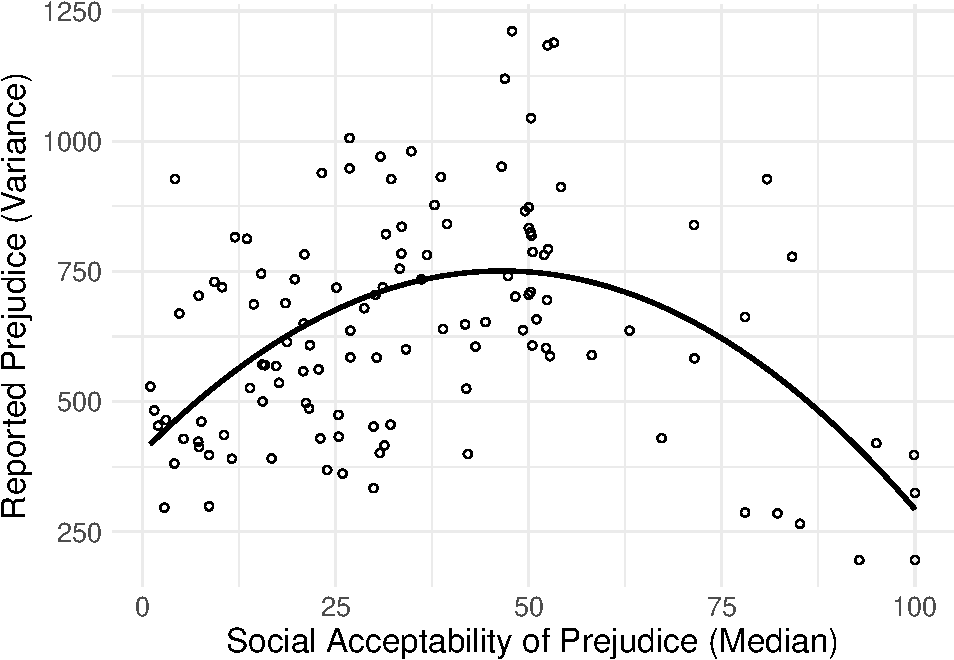
\includegraphics{beta_hurdle_files/figure-latex/unnamed-chunk-3-1.pdf}
\caption{\label{fig:unnamed-chunk-3}The stronger the normative influence on
prejudice, the smaller the variance of reported prejudice.}
\end{figure}

I also investigated normative influences on floor effects. Crandall
(1994) proposed a measure for anti-fat prejudice; in Study 5 of this
paper, Crandall makes the argument that anti-fat attitudes are more
socially acceptable (and less subject to social desirability biases)
than anti-Black prejudice. He does this by examining the decision-making
process described above with regard to hurdle models: How often do
people \emph{always} select the least prejudiced option? That is, how
often do people \emph{always} respond at the lower bound of the
distribution? He calls the proportion of people at the floor of a scale
the \enquote{politically correct (PC) index,} as this shows how often
people respond in the most socially acceptable (i.e., politically
correct) way possible. He finds that his anti-fat scale is less subject
to these floor effects: 10\% of participants always responded at the
lower bound for anti-Black prejudice, while this was only 3\% for the
anti-fat scale.

To show that norms are associated with floor effects, I calculated
Crandall's PC index for each of the 120 groups by counting how many
people responded with a 0 on the reverse-scored prejudice scale (i.e.,
\enquote{totally positive} feelings). Using a negative binomial
regression (Venables \& Ripley, 2002) for these count data, I regressed
the PC index on social acceptability of the prejudice. Perceived social
acceptability of the prejudice by one group of participants negatively
predicted the PC index, which was calculated from a \emph{separate
group} of participants, \(b = -0.03, SE = 0.002, Z = -10.97, p < .001\)
(Figure 3). The more socially acceptable a prejudice, the less people
opt for the \enquote{politically correct} floor of the scale.

\begin{figure}
\centering
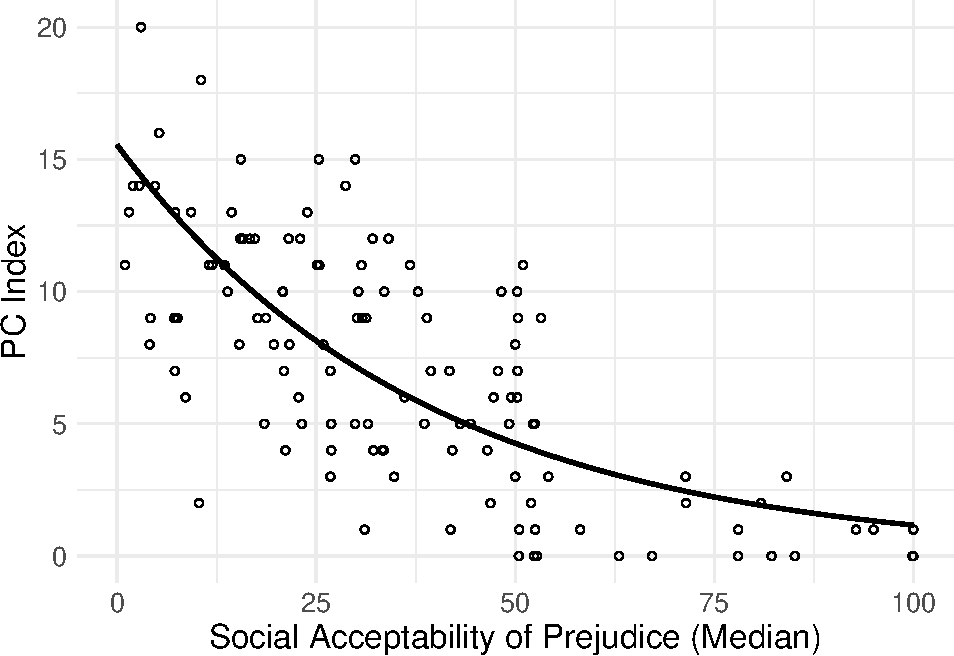
\includegraphics{beta_hurdle_files/figure-latex/unnamed-chunk-4-1.pdf}
\caption{\label{fig:unnamed-chunk-4}The more socially acceptable the
prejudice, the less people opt for the politically correct response.}
\end{figure}

This evidence shows that norms do positively predict invariance.
Predicting the scale parameter, \(\sigma\), in beta regression could be
used to investigate how much people adhere to norms regarding the
expression of certain attitudes. These data also show that normative
influence can lead to floor effects (or ceiling effects). Predicting the
shape parameters, \(\nu\) and \(\tau\), in inflated beta regression
could also be used to examine how much people adhere to norms. I now
turn to demonstrating how these beta regression models can be run in R
(R Core Team, 2017) via the \texttt{gamlss} package (Rigby \&
Stasinopoulos, 2005).

\section{Implementation in GAMLSS}\label{implementation-in-gamlss}

The \texttt{gamlss} name stands for generalized additive models for
location (i.e., \(\mu\)), scale (i.e., \(\sigma\)), and shape (i.e.,
\(\nu\) and \(\tau\)). This package gives researchers the ability to use
a wide variety of models, including beta regression models. A number of
algorithms to estimate the coefficients can be used, described in detail
by Stasinopoulos, Rigby, Heller, Voudouris, and De Bastiani (2017). To
first demonstrate how the package works according to the
parameterization discussed in the Statistical Background section, I will
generate a zero-and-one inflated beta distribution and estimate the
parameters with an intercepts-only regression using the \texttt{gamlss}
function. Then, I will demonstrate how to model social attitudes with
real data.

\subsection{Intercepts-Only
Regression}\label{intercepts-only-regression}

We can set a number of parameters for this zero-and-one inflated
distribution using the following code:

\begin{Shaded}
\begin{Highlighting}[]
\NormalTok{n <-}\StringTok{ }\DecValTok{5000}
\NormalTok{mu <-}\StringTok{ }\FloatTok{0.40}
\NormalTok{sigma <-}\StringTok{ }\FloatTok{0.60}
\NormalTok{p0 <-}\StringTok{ }\FloatTok{0.13}
\NormalTok{p1 <-}\StringTok{ }\FloatTok{0.17}
\NormalTok{p2 <-}\StringTok{ }\DecValTok{1} \OperatorTok{-}\StringTok{ }\NormalTok{p0 }\OperatorTok{-}\StringTok{ }\NormalTok{p1}
\NormalTok{a <-}\StringTok{ }\NormalTok{mu }\OperatorTok{*}\StringTok{ }\NormalTok{(}\DecValTok{1} \OperatorTok{-}\StringTok{ }\NormalTok{sigma }\OperatorTok{^}\StringTok{ }\DecValTok{2}\NormalTok{) }\OperatorTok{/}\StringTok{ }\NormalTok{(sigma }\OperatorTok{^}\StringTok{ }\DecValTok{2}\NormalTok{)}
\NormalTok{b <-}\StringTok{ }\NormalTok{a }\OperatorTok{*}\StringTok{ }\NormalTok{(}\DecValTok{1} \OperatorTok{-}\StringTok{ }\NormalTok{mu) }\OperatorTok{/}\StringTok{ }\NormalTok{mu}
\end{Highlighting}
\end{Shaded}

The sample size \texttt{n} \(= 5000\), the mean \texttt{mu} \(= 0.40\),
the scale parameter \texttt{sigma} \(= 0.60\), the probability of being
0 is \texttt{p0} \(= 0.13\), the probability of being 1 is \texttt{p1}
\(= 0.17\), and the probability of being between 0 and 1 is \texttt{p2}
\(= 1 - p_0 - p_1 = .70\). Using the equations in the Statistical
Background section, we can convert \texttt{mu} and \texttt{sigma} back
to the original shape parameters \texttt{a} (\(\alpha\)) and \texttt{b}
(\(\beta\)). The dependent variable \texttt{y} can now be generated
using the following code:

\begin{Shaded}
\begin{Highlighting}[]
\KeywordTok{set.seed}\NormalTok{(}\DecValTok{1839}\NormalTok{)}
\NormalTok{y <-}\StringTok{ }\KeywordTok{rbeta}\NormalTok{(n, a, b)}
\NormalTok{cat <-}\StringTok{ }\KeywordTok{sample}\NormalTok{(}\DecValTok{1}\OperatorTok{:}\DecValTok{3}\NormalTok{, n, }\DataTypeTok{prob =} \KeywordTok{c}\NormalTok{(p0, p2, p1), }\DataTypeTok{replace =} \OtherTok{TRUE}\NormalTok{)}
\NormalTok{y[cat }\OperatorTok{==}\StringTok{ }\DecValTok{1}\NormalTok{] <-}\StringTok{ }\DecValTok{0}
\NormalTok{y[cat }\OperatorTok{==}\StringTok{ }\DecValTok{3}\NormalTok{] <-}\StringTok{ }\DecValTok{1}
\end{Highlighting}
\end{Shaded}

I draw \texttt{n} random numbers from the beta distribution with shape
parameters \texttt{a} and \texttt{b}. I then draw \texttt{n} numbers
ranging from 1 to 3 with probabilities \texttt{p0}, \texttt{p2}, and
\texttt{p1}, respectively. If 1 was drawn, that observation is 0; if 2
was drawn, it remains being from the beta distribution; if 3 was drawn,
that observation is 1. In this way, \texttt{p0}, \texttt{p2}, and
\texttt{p1} determine the probability of being 0, from a beta
distribution, or being 1, respectively.

The \texttt{gamlss} function has four arguments for formulas---one for
each of the parameters. It also has an argument, \texttt{family}, that
determines what distribution will be used in fitting the model. For a
zero-and-one inflated beta regression, the family is \texttt{BEINF()}.
One can fit the intercepts-only model using the following code:

\begin{Shaded}
\begin{Highlighting}[]
\NormalTok{fit <-}\StringTok{ }\KeywordTok{gamlss}\NormalTok{(}
  \DataTypeTok{formula =}\NormalTok{ y }\OperatorTok{~}\StringTok{ }\DecValTok{1}\NormalTok{,     }\CommentTok{# formula for mu}
  \DataTypeTok{formula.sigma =} \OperatorTok{~}\StringTok{ }\DecValTok{1}\NormalTok{, }\CommentTok{# formula for sigma}
  \DataTypeTok{formula.nu =} \OperatorTok{~}\StringTok{ }\DecValTok{1}\NormalTok{,    }\CommentTok{# formula for nu}
  \DataTypeTok{formula.tau =} \OperatorTok{~}\StringTok{ }\DecValTok{1}\NormalTok{,   }\CommentTok{# formula for tau}
  \DataTypeTok{family =} \KeywordTok{BEINF}\NormalTok{()     }\CommentTok{# distribution for model}
\NormalTok{)}
\end{Highlighting}
\end{Shaded}

One can use the inverse link functions to transform the coefficients
back into the original scale as to compare them to the parameters set
above. The estimated parameters are calculated using the following code,
according to the equations and link functions described in the
Statistical Background section:

\begin{Shaded}
\begin{Highlighting}[]
\NormalTok{inv_logit <-}\StringTok{ }\ControlFlowTok{function}\NormalTok{(x) }\KeywordTok{exp}\NormalTok{(x) }\OperatorTok{/}\StringTok{ }\NormalTok{(}\DecValTok{1} \OperatorTok{+}\StringTok{ }\KeywordTok{exp}\NormalTok{(x)) }\CommentTok{# inverse of link function}
\NormalTok{fit_mu <-}\StringTok{ }\KeywordTok{inv_logit}\NormalTok{(fit}\OperatorTok{$}\NormalTok{mu.coefficients)}
\NormalTok{fit_sigma <-}\StringTok{ }\KeywordTok{inv_logit}\NormalTok{(fit}\OperatorTok{$}\NormalTok{sigma.coefficients)}
\NormalTok{fit_nu <-}\StringTok{ }\KeywordTok{exp}\NormalTok{(fit}\OperatorTok{$}\NormalTok{nu.coefficients)}
\NormalTok{fit_tau <-}\StringTok{ }\KeywordTok{exp}\NormalTok{(fit}\OperatorTok{$}\NormalTok{tau.coefficients)}
\NormalTok{fit_p0 <-}\StringTok{ }\NormalTok{fit_nu }\OperatorTok{/}\StringTok{ }\NormalTok{(}\DecValTok{1} \OperatorTok{+}\StringTok{ }\NormalTok{fit_nu }\OperatorTok{+}\StringTok{ }\NormalTok{fit_tau)}
\NormalTok{fit_p1 <-}\StringTok{ }\NormalTok{fit_tau }\OperatorTok{/}\StringTok{ }\NormalTok{(}\DecValTok{1} \OperatorTok{+}\StringTok{ }\NormalTok{fit_nu }\OperatorTok{+}\StringTok{ }\NormalTok{fit_tau)}
\end{Highlighting}
\end{Shaded}

The estimates for \(\mu\), \(\sigma\), \(p_0\), and \(p_1\) are
\(.406\), \(.597\), \(.136\), and \(.171\), respectively. These are
close estimates to the population parameters set above. In research
settings, each of the parameters would not be set to one number (i.e.,
an intercept), but be regressed on observed variables of theoretical
interest. For an exaample, I now turn to a model using real data.

\subsection{Modeling Political
Ideology}\label{modeling-political-ideology}

The social dominance orientation (SDO) scale measures how much one
supports social hierarchy and inequality in society (Ho et al., 2015;
Pratto, Sidanius, Stallworth, \& Malle, 1994). In personality
psychology, it has a robust, oft-replicated positive relationship with
political conservatism (Duriez \& Van Hiel, 2002; Hiel \& Mervielde,
2002; Ho et al., 2015; Pratto et al., 2000; Pratto, Stallworth, \&
Conway-Lanz, 1998; Pratto, Stallworth, \& Sidanius, 1997; Wilson \&
Sibley, 2013). Some consider SDO a central aspect of contemporary
American conservatism (Eidelman, Crandall, Goodman, \& Blanchar, 2012;
Jost, Glaser, Kruglanski, \& Sulloway, 2003). However, openly admitting
that some groups are inherently better than others is a socially
unacceptable thing to express, often leading to floor effects. I regress
SDO on conservatism in both an OLS and beta regression framework to
compare and contrast the two methods.

The data come from Study 1 of White and Crandall (2017), where 175
participants answered an 8-item, 7-point SDO scale (Ho et al., 2015) and
two 7-point items that assessed conservatism (i.e., Democrat, 1, to
Republican, 7, and liberal, 1, to conservative, 7). Scales were
calculated by averaging their respective items. Figure 4 shows the
histogram of the SDO scale---30\% of the sample responded with 1s for
each of the 8 items, demonstrating a floor effect.

\begin{figure}
\centering
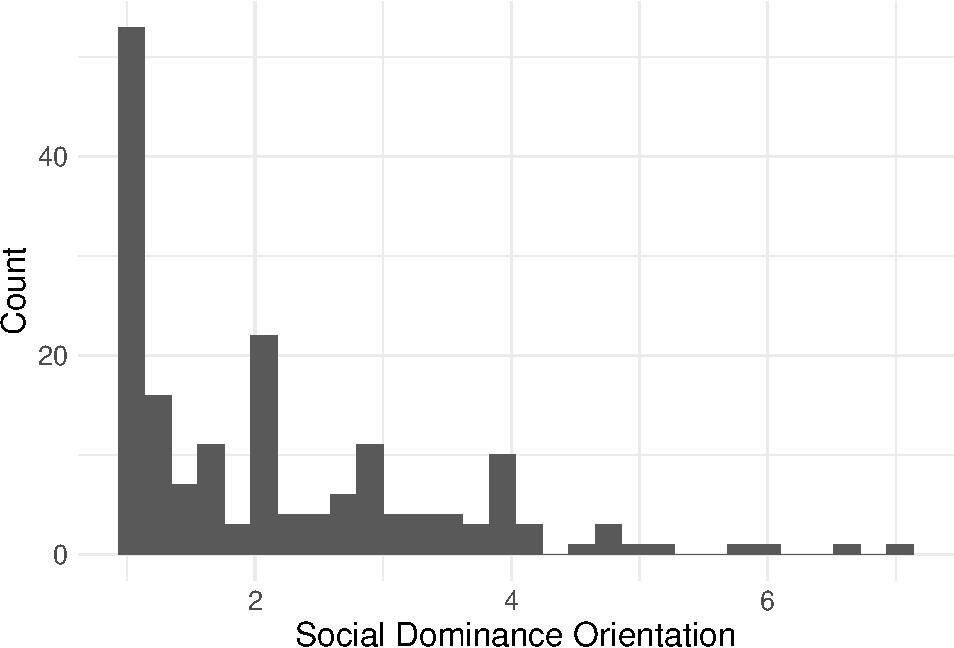
\includegraphics{beta_hurdle_files/figure-latex/unnamed-chunk-11-1.pdf}
\caption{\label{fig:unnamed-chunk-11}The distribution of SDO scores contains
a floor effect.}
\end{figure}

The two variables correlated at \(r = .50, p < .001\). Figure 5 shows
the predicted values against the standardized residuals from regressing
SDO on conservatism using OLS, with a marginal histogram showing the
distribution of residuals. A loess line is drawn, and a slight jitter
has been added to the points, given that many points overlapped with one
another. One can see a spread of residuals getting wider as predicted
values increases, suggesting heteroskedasticity; moreover, the histogram
shows that the residuals are positively skewed, violating the assumption
of conditional normality. How does this compare with beta regression?

\begin{figure}
\centering
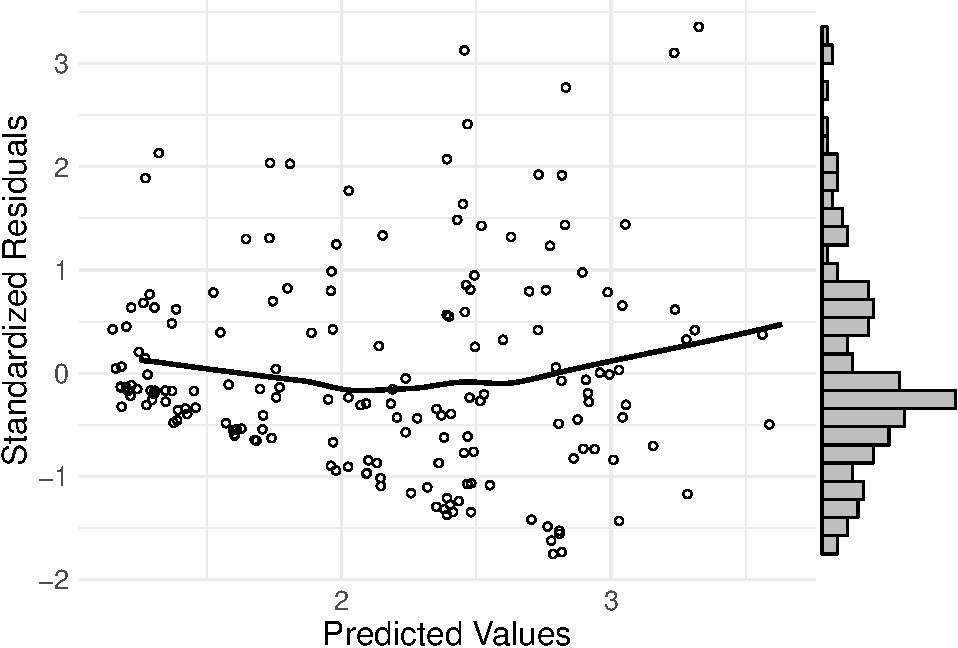
\includegraphics{beta_hurdle_files/figure-latex/unnamed-chunk-12-1.pdf}
\caption{\label{fig:unnamed-chunk-12}The residuals plot shows
heteroskedasticity and conditional non-normality.}
\end{figure}

First, I need to rescale the data. SDO was measured on a 1-to-7 scale,
so \(l = 1\) and \(u = 7\). One can use the following R code to rescale
a variable to \(0 \leq y \leq 1\), following the equation described in
the Modeling Bounded Variables Beyond the Zero Through One Range
section:

\begin{Shaded}
\begin{Highlighting}[]
\NormalTok{dat}\OperatorTok{$}\NormalTok{sdo <-}\StringTok{ }\NormalTok{(dat}\OperatorTok{$}\NormalTok{sdo }\OperatorTok{-}\StringTok{ }\DecValTok{1}\NormalTok{) }\OperatorTok{/}\StringTok{ }\NormalTok{(}\DecValTok{7} \OperatorTok{-}\StringTok{ }\DecValTok{1}\NormalTok{)}
\end{Highlighting}
\end{Shaded}

It is important to remember that \(l\) and \(u\) are \emph{not} the
minimum and maximum \emph{observed} values, but the minimum and maximum
\emph{possible} values; for example, if lowest SDO score observed was 2,
\(l\) would still be 1.

\begin{table}[tbp]
\begin{center}
\begin{threeparttable}
\caption{\label{tab:unnamed-chunk-14}Guide for Choosing Correct Distribution and Corresponding gamlss Family}
\begin{tabular}{lllll}
\toprule
Any $y_i = 0$? & Any $y_i = 1$? & Distribution & gamlss Family & Submodels\\
\midrule
No & No & Beta & BE() & $\mu$, $\sigma$\\
Yes & No & Zero-Inflated Beta & BEINF0() & $\mu$, $\sigma$, $\nu$\\
No & Yes & One-Inflated Beta & BEINF1() & $\mu$, $\sigma$, $\nu$\\
Yes & Yes & Zero-and-One Inflated Beta & BEINF() & $\mu$, $\sigma$, $\nu$, $\tau$\\
\bottomrule
\end{tabular}
\end{threeparttable}
\end{center}
\end{table}

The last thing a researcher has to do is decide which value to use for
the \texttt{family} argument in the \texttt{gamlss} function.
Researchers can follow Table 1 for deciding which value is appropriate.
One can check to see the minimum and maximum observed by using the
\texttt{range()} function in R. In this case, \texttt{range(dat\$sdo)}
returns \texttt{0\ 1}, showing that both 0s and 1s are observed.
According to Table 1, I should use \texttt{BEINF()} for the
\texttt{family}. I run the beta regression model, using conservatism
(i.e., \texttt{rw\_polid}) to predict all four parameters, with the
following code:

\begin{Shaded}
\begin{Highlighting}[]
\NormalTok{fit_beinf <-}\StringTok{ }\KeywordTok{gamlss}\NormalTok{(sdo }\OperatorTok{~}\StringTok{ }\NormalTok{rw_polid, }\OperatorTok{~}\StringTok{ }\NormalTok{rw_polid, }\OperatorTok{~}\StringTok{ }\NormalTok{rw_polid, }\OperatorTok{~}\StringTok{ }\NormalTok{rw_polid,}
                    \DataTypeTok{data =}\NormalTok{ dat, }\DataTypeTok{family =} \KeywordTok{BEINF}\NormalTok{())}
\end{Highlighting}
\end{Shaded}

Finally, one can use the \texttt{summary()} function to examine the
results. Table 2 shows the coefficients tables for each of the four
submodels from the summary. The \(\mu\) submodel tells the same story as
the OLS model: The more conservative one is, the more they support
hierarchy in society \(b = 0.28, SE = 0.05, t(167) = 5.46, p < .001\).
Since a logistic link function is used, however, this relationship is
not linear (see Figure 7). The \(\sigma\) submodel shows that, as people
get more conservative, they also display more variance in their
responses to the SDO scale,
\(b = 0.14, SE = 0.06, t(167) = 2.48, p = .014\); conservatives are not
just more supportive of hierarchy, they also display a wider range of
attitudes toward hierarchy. In line with the evidence presented above
that norms produce invariance, one explanation for this relationship is
that conservatives are less influenced by norms against expressing
attitudes in favor of social inequality. The conservatism coefficient
for the \(\nu\) model is also significant: The more conservatism one
reports, the less likely they are to respond at the floor (i.e., in a
``politically correct'' manner; Crandall, 1994),
\(b = -0.54, SE = 0.12, t(167) = -4.46, p < .001\). Again, an
interpretation here is that conservatives are less influenced by the
normative pressure to completely reject social inequality and group
hierarchies. Lastly, the coefficient for the \(\tau\) submodel is not
significant; however, this could be an issue of statistical power, given
that only one participant responded at the ceiling.

\begin{table}[tbp]
\begin{center}
\begin{threeparttable}
\caption{\label{tab:unnamed-chunk-17}Results From the Beta Regression Model}
\begin{tabular}{llrrrr}
\toprule
Submodel & Variable & $b$ & $SE$ & $t$ & $p$\\
\midrule
$\mu$ & Intercept & -2.03 & 0.20 & -10.15 & < .001\\
 & Conservatism & 0.28 & 0.05 & 5.46 & < .001\\
$\sigma$ & Intercept & -0.97 & 0.22 & -4.42 & < .001\\
 & Conservatism & 0.14 & 0.06 & 2.48 & .014\\
$\nu$ & Intercept & 0.82 & 0.38 & 2.13 & .034\\
 & Conservatism & -0.54 & 0.12 & -4.46 & < .001\\
$\tau$ & Intercept & -13.33 & 6.91 & -1.93 & .055\\
 & Conservatism & 1.70 & 1.15 & 1.47 & .143\\
\bottomrule
\end{tabular}
\end{threeparttable}
\end{center}
\end{table}

How do the OLS and beta regression results compare? Figure 6 shows a
scatterplot of SDO regressed onto conservatism using OLS regression. The
solid line is the regression line. The estimated standard deviation of
the residuals, \(\sigma_\epsilon\), is added to and subtracted from this
line; these are the dotted lines. In line with the assumption of
homoskedasticity, this standard deviation is constant across all levels
of conservatism. Importantly, the lower dotted line dips below possible
observed values---the model assumes that predicted values come from a
distribution that has values in it that \emph{cannot} be observed with
the Likert scale used.

\begin{figure}
\centering
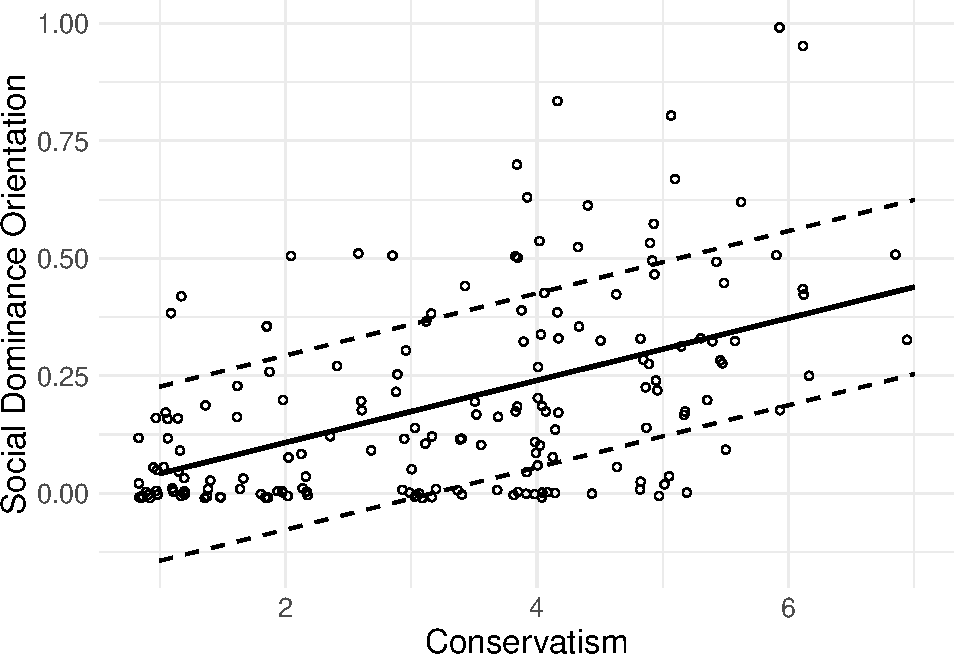
\includegraphics{beta_hurdle_files/figure-latex/unnamed-chunk-18-1.pdf}
\caption{\label{fig:unnamed-chunk-18}SDO regressed on conservatism, using
OLS regression. Dotted lines are one standard deviation (i.e., estimated
standard deviation of the residuals) above and below the solid
regression line.}
\end{figure}

Figure 7 shows the same figure for the zero-and-one inflated beta
regression model. The width of the dotted line increases as conservatism
increases, demonstrating the heteroskedasticity of the model. This also
shows that variance in SDO scores increases with conservatism; also note
that the dotted line does not dip below the floor, as values in the beta
distribution cannot be less than the lower bound.

\begin{figure}
\centering
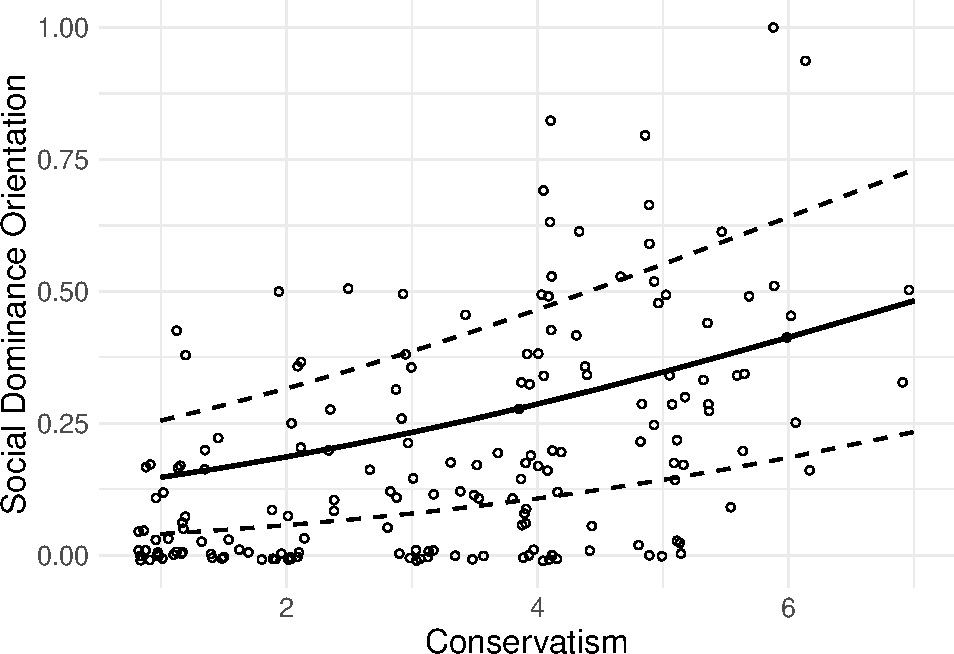
\includegraphics{beta_hurdle_files/figure-latex/unnamed-chunk-19-1.pdf}
\caption{\label{fig:unnamed-chunk-19}SDO regressed on conservatism, using
beta regression. Dotted lines are one standard deviation (i.e.,
estimated standard deviation of the residuals) above and below the solid
regression line.}
\end{figure}

\subsection{Diagnostic Checks and Other Models with Conditional
Variance}\label{diagnostic-checks-and-other-models-with-conditional-variance}

Diagnostic checks---such as inspecting the residuals---for beta
regression models is still an active area of research, with many
different authors proposing different techniques for diagnosing issues
with these models (Espinheira, Ferrari, \& Cribari-Neto, 2008b, 2008a;
Espinheira, Santos, \& Cribari-Neto, 2017; Pereira, 2017). There does
not seem yet to be an agreed-upon method for performing diagnostic
checks on these models.

Beta regression can also be implemented in the \texttt{betareg} package
(Cribari-Neto \& Zeileis, 2010; Grün, Kosmidis, \& Zeileis, 2012), but
it does not allow for modeling zeros and ones as easily. The
\texttt{ZOIP} package (Diaz Zapata, 2017) is also available, which can
be used to model mixed effects. Both of these packages use a separate
parameterization than the \texttt{gamlss} package. Beta regression is
not the only way to model conditional variance---I chose to focus on the
method here because it is a flexible distribution that handles a large
range of non-normal shapes. Dispersion can also be predicted using
double generalized linear models in the \texttt{dglm} R package (Smyth,
1989; Smyth \& Verbyla, 1999) or heteroskedastic censored and truncated
regression using the \texttt{crch} R package (Messner, Mayr, \& Zeileis,
2016; Messner, Zeileis, Broecker, \& Mayr, 2014), among others.

\section{Conclusion}\label{conclusion}

Common statistial procedures that assume normality and homoskedasticity
ignore interesting theoretical phenomena in data. I described the beta
regression, demonstrated that norms can produce invariance, and provided
a tutorial on how to fit numerous beta-regression models using free
statistical software. Louis et al. (2003) argued that common statistical
procedures (a) motivate researchers to seek out measures that match the
assumptions of common statistical procedures, allowing the tools we use
to influence the phenomena we study, and (b) provide a misleading
picture of the relationships between variables that are strongly
influenced by norms. I believe beta regression can be a useful tool for
addressing these issues.

\newpage

\section{References}\label{references}

\setlength{\parindent}{-0.5in} \setlength{\leftskip}{0.5in}

\hypertarget{refs}{}
\hypertarget{ref-abdel2017extended}{}
Abdel-Karim, A. H. (2017). Extended zero-one inflated beta and adjusted
three-part regression models for proportional data analysis.
\emph{Communications in Statistics - Simulation and Computation},
\emph{46}(8), 6155--6172.

\hypertarget{ref-buntaine2011does}{}
Buntaine, M. T. (2011). Does the Asian Development Bank respond to past
environmental performance when allocating environmentally risky
financing? \emph{World Development}, \emph{39}(3), 336--350.

\hypertarget{ref-cameron2005microeconometrics}{}
Cameron, A. C., \& Trivedi, P. K. (2005). \emph{Microeconometrics:
Methods and applications}. New York, NY: Cambridge University Press.

\hypertarget{ref-carlevaro2016multiple}{}
Carlevaro, F., Croissant, Y., \& Hoareau, S. (2017). \emph{Multiple
hurdle Tobit models in R: The mhurdle package}. Retrieved from
\url{https://cran.r-project.org/web/packages/mhurdle/vignettes/mhurdle.pdf}

\hypertarget{ref-cary2014prevalence}{}
Cary, L. A., \& Page-Gould, E. (2014). The prevalence and impact of
sexism, racism and homophobia in online gaming environments. Poster
presented at the annual meeting of the Society for Personality and
Social Psychology, Austin, TX.

\hypertarget{ref-coxe2013generalized}{}
Coxe, S., West, S. G., \& Aiken, L. S. (2013). Generalized linear
models. In T. D. Little (Ed.), \emph{The Oxford handbook of quantitative
methods, Volume II} (pp. 26--51). New York, NY: Oxford University Press.

\hypertarget{ref-cragg1971some}{}
Cragg, J. G. (1971). Some statistical models for limited dependent
variables with application to the demand for durable goods.
\emph{Econometrica: Journal of the Econometric Society}, \emph{39}(5),
829--844.

\hypertarget{ref-crandall1994prejudice}{}
Crandall, C. S. (1994). Prejudice against fat people: Ideology and
self-interest. \emph{Journal of Personality and Social Psychology},
\emph{66}(5), 882--894.

\hypertarget{ref-crandall2002social}{}
Crandall, C. S., Eshleman, A., \& O'Brien, L. (2002). Social norms and
the expression and suppression of prejudice: The struggle for
internalization. \emph{Journal of Personality and Social Psychology},
\emph{82}(3), 359--378.

\hypertarget{ref-cribarineto2010beta}{}
Cribari-Neto, F., \& Zeileis, A. (2010). Beta regression in R.
\emph{Journal of Statistical Software}, \emph{34}(2).

\hypertarget{ref-zoip2017}{}
Diaz Zapata, J. C. (2017). \emph{ZOIP: ZOIP distribution, ZOIP
regression, ZOIP mixed regression}. Retrieved from
\url{https://CRAN.R-project.org/package=ZOIP}

\hypertarget{ref-duriez2002march}{}
Duriez, B., \& Van Hiel, A. (2002). The march of modern fascism: A
comparison of social dominance orientation and authoritarianism.
\emph{Personality and Individual Differences}, \emph{32}(7), 1199--1213.

\hypertarget{ref-eidelman2012low}{}
Eidelman, S., Crandall, C. S., Goodman, J. A., \& Blanchar, J. C.
(2012). Low-effort thought promotes political conservatism.
\emph{Personality and Social Psychology Bulletin}, \emph{38}(6),
808--820.

\hypertarget{ref-eskelson2011estimating}{}
Eskelson, B. N., Madsen, L., Hagar, J. C., \& Temesgen, H. (2011).
Estimating riparian understory vegetation cover with beta regression and
copula models. \emph{Forest Science}, \emph{57}(3), 212--221.

\hypertarget{ref-espinheira2008influence}{}
Espinheira, P. L., Ferrari, S. L., \& Cribari-Neto, F. (2008a).
Influence diagnostics in beta regression. \emph{Computational Statistics
\& Data Analysis}, \emph{52}(9), 4417--4431.

\hypertarget{ref-espinheira2008beta}{}
Espinheira, P. L., Ferrari, S. L., \& Cribari-Neto, F. (2008b). On beta
regression residuals. \emph{Journal of Applied Statistics},
\emph{35}(4), 407--419.

\hypertarget{ref-espinheira2017nonlinear}{}
Espinheira, P. L., Santos, E. G., \& Cribari-Neto, F. (2017). On
nonlinear beta regression residuals. \emph{Biometrical Journal},
\emph{59}(3), 445--461.

\hypertarget{ref-everitt2002cambridge}{}
Everitt, B., \& Skrondal, A. (2010). \emph{The Cambridge dictionary of
statistics}. New York, NY: Cambridge University Press.

\hypertarget{ref-ferrari2004beta}{}
Ferrari, S. L., \& Cribari-Neto, F. (2004). Beta regression for
modelling rates and proportions. \emph{Journal of Applied Statistics},
\emph{31}(7), 799--815.

\hypertarget{ref-gallardo2012analysis}{}
Gallardo, A., Bovea, M. D., Colomer, F. J., \& Prades, M. (2012).
Analysis of collection systems for sorted household waste in Spain.
\emph{Waste Management}, \emph{32}(9), 1623--1633.

\hypertarget{ref-grun2012extended}{}
Grün, B., Kosmidis, I., \& Zeileis, A. (2012). Extended beta regression
in R: Shaken, stirred, mixed, and partitioned. \emph{Journal of
Statistical Software}, \emph{48}(11).

\hypertarget{ref-hayes2007using}{}
Hayes, A. F., \& Cai, L. (2007). Using heteroskedasticity-consistent
standard error estimators in OLS regression: An introduction and
software implementation. \emph{Behavior Research Methods}, \emph{39}(4),
709--722.

\hypertarget{ref-hiel2002explaining}{}
Hiel, A. V., \& Mervielde, I. (2002). Explaining conservative beliefs
and political preferences: A comparison of social dominance orientation
and authoritarianism. \emph{Journal of Applied Social Psychology},
\emph{32}(5), 965--976.

\hypertarget{ref-ho2015nature}{}
Ho, A. K., Sidanius, J., Kteily, N., Sheehy-Skeffington, J., Pratto, F.,
Henkel, K. E., \ldots{} Stewart, A. L. (2015). The nature of social
dominance orientation: Theorizing and measuring preferences for
intergroup inequality using the new SDO\(_7\) scale. \emph{Journal of
Personality and Social Psychology}, \emph{109}(6), 1003--1028.

\hypertarget{ref-hubben2008societal}{}
Hubben, G. A. A., Bishai, D., Pechlivanoglou, P., Cattelan, A. M.,
Grisetti, R., Facchin, C., \ldots{} Tramarin, A. (2008). The societal
burden of HIV/AIDS in Northern Italy: An analysis of costs and quality
of life. \emph{AIDS Care}, \emph{20}(4), 449--455.

\hypertarget{ref-jost2003political}{}
Jost, J. T., Glaser, J., Kruglanski, A. W., \& Sulloway, F. J. (2003).
Political conservatism as motivated social cognition.
\emph{Psychological Bulletin}, \emph{129}(3), 339--375.

\hypertarget{ref-lewin1951field}{}
Lewin, K. (1951). \emph{Field theory in social science: Selected
theoretical papers}. (D. Cartwright, Ed.). New York, NY: Harper \& Row.

\hypertarget{ref-long2000using}{}
Long, J. S., \& Ervin, L. H. (2000). Using heteroscedasticity consistent
standard errors in the linear regression model. \emph{The American
Statistician}, \emph{54}(3), 217--224.

\hypertarget{ref-louis2003reflections}{}
Louis, W. R., Mavor, K. I., \& Terry, D. J. (2003). Reflections on the
statistical analysis of personality and norms in war, peace, and
prejudice: Are deviant minorities the problem? \emph{Analyses of Social
Issues and Public Policy}, \emph{3}(1), 189--198.

\hypertarget{ref-mcbee2010modeling}{}
McBee, M. (2010). Modeling outcomes with floor or ceiling effects: An
introduction to the tobit model. \emph{Gifted Child Quarterly},
\emph{54}(4), 314--320.

\hypertarget{ref-messner2016heteroscedastic}{}
Messner, J. W., Mayr, G. J., \& Zeileis, A. (2016). Heteroscedastic
censored and truncated regression with crch. \emph{The R Journal},
\emph{8}(1), 173--181.

\hypertarget{ref-messner2014probabilistic}{}
Messner, J. W., Zeileis, A., Broecker, J., \& Mayr, G. J. (2014).
Probabilistic wind power forecasts with an inverse power curve
transformation and censored regression. \emph{Wind Energy},
\emph{17}(11), 1753--1766.

\hypertarget{ref-ospina2010inflated}{}
Ospina, R., \& Ferrari, S. L. (2010). Inflated beta distributions.
\emph{Statistical Papers}, \emph{51}(1), 111--126.

\hypertarget{ref-peplonska2012rotating}{}
Peplonska, B., Bukowska, A., Sobala, W., Reszka, E., Gromadzińska, J.,
Wasowicz, W., \ldots{} Ursin, G. (2012). Rotating night shift work and
mammographic density. \emph{Cancer, Epidemiology, Biomarkers, \&
Prevention}, \emph{21}(7), 1028--1037.

\hypertarget{ref-pereira2017quantile}{}
Pereira, G. H. (2017). On quantile residuals in beta regression.
\emph{Communications in Statistics - Simulation and Computation}, 1--15.

\hypertarget{ref-pratto2000social}{}
Pratto, F., Liu, J. H., Levin, S., Sidanius, J., Shih, M., Bachrach, H.,
\& Hegarty, P. (2000). Social dominance orientation and the
legitimization of inequality across cultures. \emph{Journal of
Cross-Cultural Psychology}, \emph{31}(3), 369--409.

\hypertarget{ref-pratto1994social}{}
Pratto, F., Sidanius, J., Stallworth, L. M., \& Malle, B. F. (1994).
Social dominance orientation: A personality variable predicting social
and political attitudes. \emph{Journal of Personality and Social
Psychology}, \emph{67}(4), 741--763.

\hypertarget{ref-pratto1998social}{}
Pratto, F., Stallworth, L. M., \& Conway-Lanz, S. (1998). Social
dominance orientation and the ideological legitimization of social
policy. \emph{Journal of Applied Social Psychology}, \emph{28}(20),
1853--1875.

\hypertarget{ref-pratto1997gender}{}
Pratto, F., Stallworth, L. M., \& Sidanius, J. (1997). The gender gap:
Differences in political attitudes and social dominance orientation.
\emph{British Journal of Social Psychology}, \emph{36}(1), 49--68.

\hypertarget{ref-rcore2017}{}
R Core Team. (2017). \emph{R: A language and environment for statistical
computing}. Vienna, Austria: R Foundation for Statistical Computing.
Retrieved from \url{https://www.R-project.org/}

\hypertarget{ref-rigby2005generalized}{}
Rigby, R. A., \& Stasinopoulos, D. M. (2005). Generalized additive
models for location, scale and shape, (with discussion). \emph{Applied
Statistics}, \emph{54}(3), 507--554.

\hypertarget{ref-rigby2017distributions}{}
Rigby, R. A., Stasinopoulos, D. M., Heller, G., \& De Bastiani, F.
(2017). \emph{Distributions for modelling location, scale, and shape:
Using GAMLSS in R. Unpublished draft}. Retrieved from
\url{gamlss.com/books-articles}

\hypertarget{ref-rosopa2013managing}{}
Rosopa, P. J., Schaffer, M. M., \& Schroeder, A. N. (2013). Managing
heteroscedasticity in general linear models. \emph{Psychological
Methods}, \emph{18}(3), 335--351.

\hypertarget{ref-smithson2013generalized}{}
Smithson, M., \& Merkle, E. C. (2013). \emph{Generalized linear models
for categorical and continuous limited dependent variables}. Boca Raton,
FL: CRC Press.

\hypertarget{ref-smithson2006better}{}
Smithson, M., \& Verkuilen, J. (2006). A better lemon squeezer?
Maximum-likelihood regression with beta-distributed dependent variables.
\emph{Psychological Methods}, \emph{11}(1), 54--71.

\hypertarget{ref-smyth1989generalized}{}
Smyth, G. K. (1989). Generalized linear models with varying dispersion.
\emph{Journal of the Royal Statistical Society. Series B
(Methodological)}, \emph{51}(1), 47--60.

\hypertarget{ref-smyth1999adjusted}{}
Smyth, G. K., \& Verbyla, A. P. (1999). Adjusted likelihood methods for
modelling dispersion in generalized linear models.
\emph{Environmetrics}, \emph{10}(6), 695--709.

\hypertarget{ref-stasinopoulos2017flexible}{}
Stasinopoulos, D. M., Rigby, R. A., Heller, G. Z., Voudouris, V., \& De
Bastiani, F. (2017). \emph{Flexible regression and smoothing: Using
GAMLSS in R}. Boca Raton, FL: CRC Press.

\hypertarget{ref-venables2002modern}{}
Venables, W. N., \& Ripley, B. D. (2002). \emph{Modern applied
statistics with S}. New York, NY: Springer.

\hypertarget{ref-white2017freedom}{}
White, M. H., II, \& Crandall, C. S. (2017). Freedom of racist speech:
Ego and expressive threats. \emph{Journal of Personality and Social
Psychology}, \emph{113}(3), 413--429.

\hypertarget{ref-wilson2013social}{}
Wilson, M. S., \& Sibley, C. G. (2013). Social dominance orientation and
right-wing authoritarianism: Additive and interactive effects on
political conservatism. \emph{Political Psychology}, \emph{34}(2),
277--284.

\hypertarget{ref-wooldridge2010econometric}{}
Wooldridge, J. M. (2010). \emph{Econometric analysis of cross section
and panel data}. Cambridge, MA: MIT Press.






\end{document}
